\section{Fase 1. Evaluación del sistema original}
\label{sec:resultados_fase1}

Se identificaron deficiencias mecánicas en los mecanismos de traslación de los ejes X, Y y Z. La configuración inicial incorporó tubos metálicos para instalaciones eléctricas como elementos de guiado y carros impresos en 3D con rodamientos radiales de bolas (Figura~\ref{fig:fase1_vista_general}).

\begin{figure}[H]
    \centering
    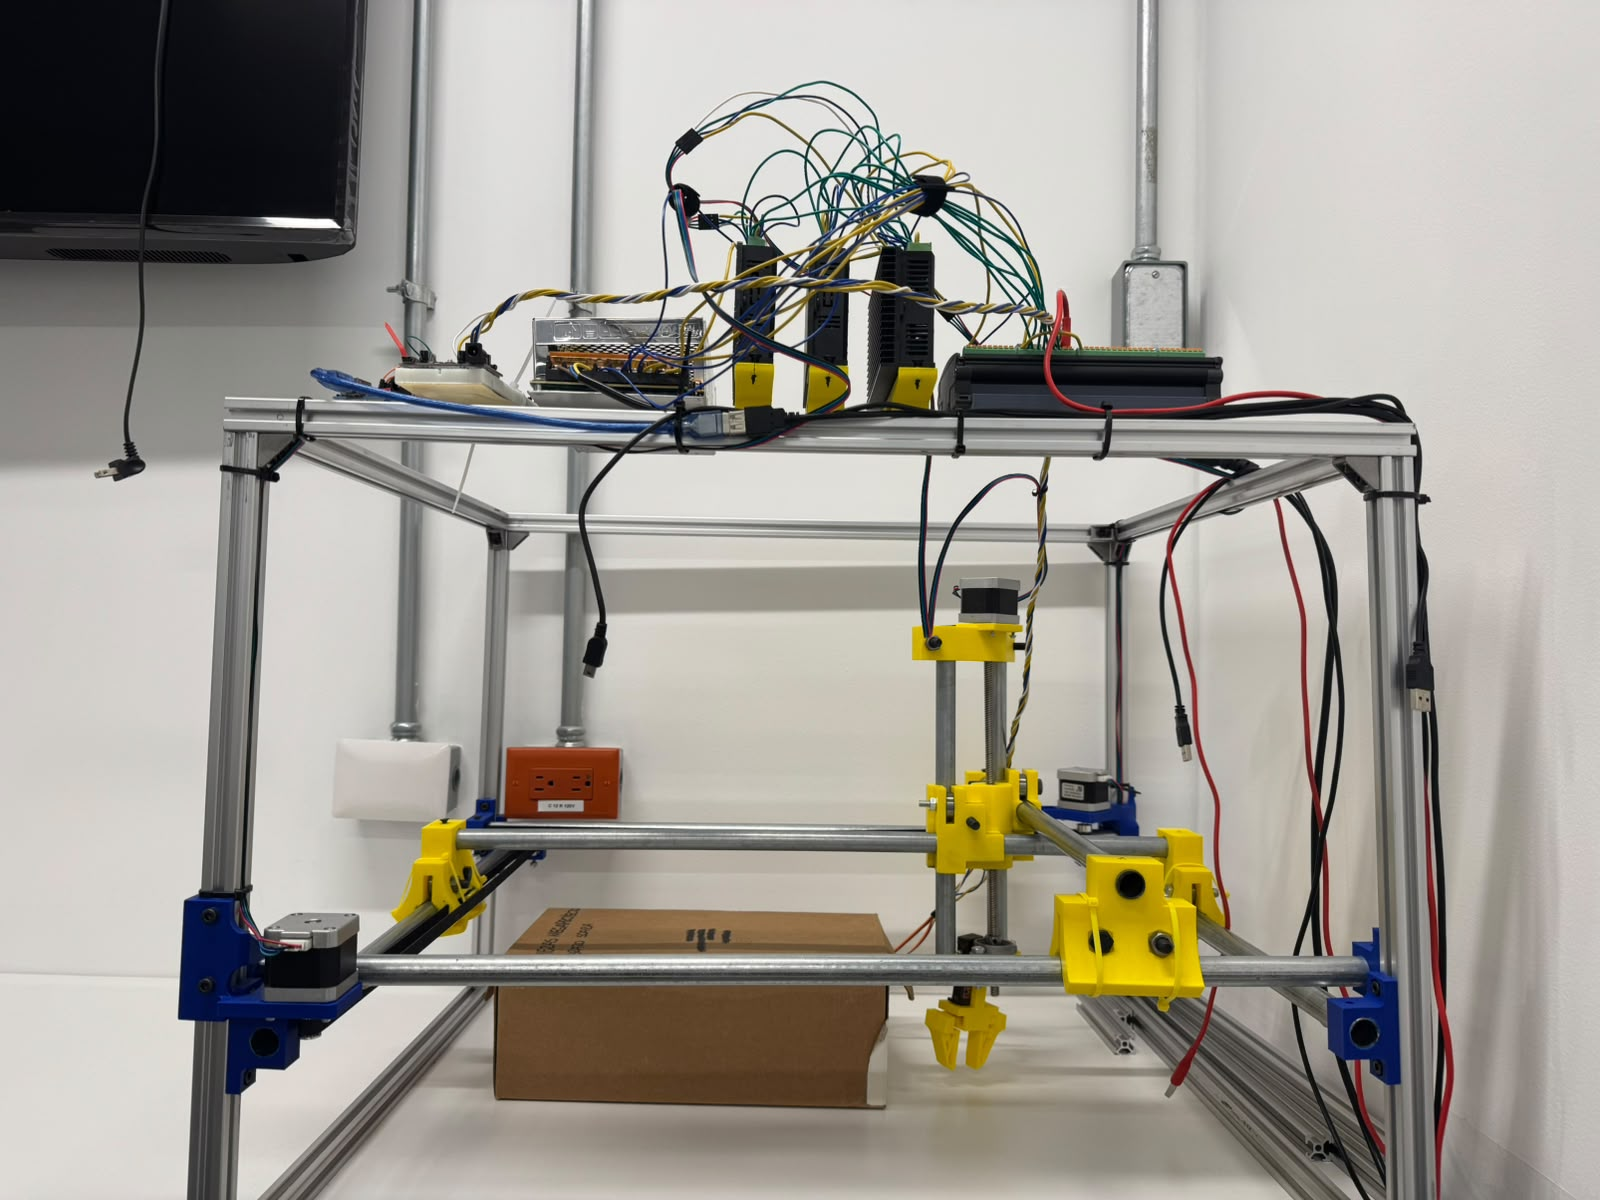
\includegraphics[width=0.75\textwidth,height=6cm,keepaspectratio]{Imagenes de Documentacion/F1_1.jpeg}
    \caption{Configuración inicial del brazo robótico cartesiano.}
    \label{fig:fase1_vista_general}
    \par\small Fuente: elaboración propia.
\end{figure}

En los cuatro carros de X y Y se observó resistencia al desplazamiento y falta de alineación con las guías. También se identificó contacto entre las piezas plásticas y los tubos (Figura~\ref{fig:fase1_carro_xy}). Durante el movimiento del pórtico se observó un avance desigual de sus extremos, identificado como \textit{gantry racking}.

\begin{figure}[H]
    \centering
    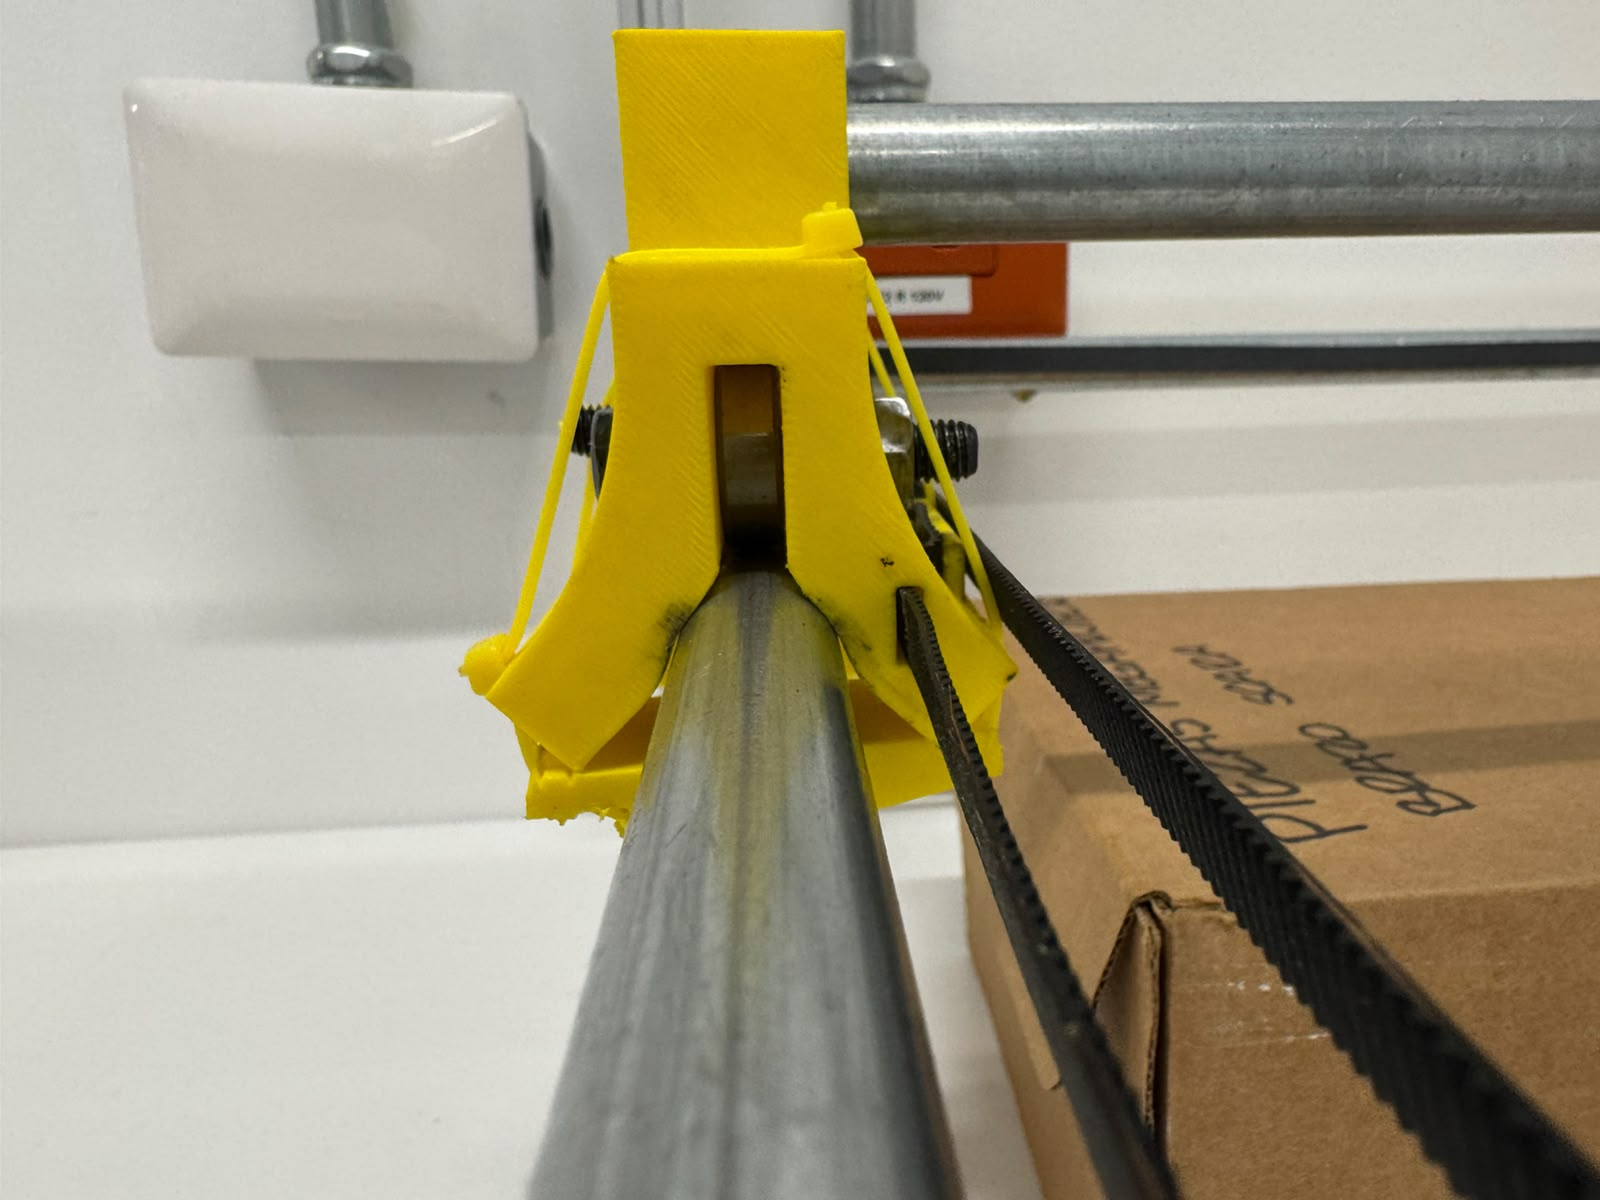
\includegraphics[width=0.65\textwidth,height=5.5cm,keepaspectratio]{Imagenes de Documentacion/F1_3.jpeg}
    \caption{Carro y elementos de guiado del sistema original en X y Y.}
    \label{fig:fase1_carro_xy}
    \par\small Fuente: elaboración propia.
\end{figure}

En Z se observó desalineación del conjunto móvil respecto a la dirección vertical. La disposición del motor, el mecanismo de desplazamiento y la garra se documentó en la Figura~\ref{fig:fase1_eje_z}. Las observaciones de la inspección manual se resumieron en el Cuadro~\ref{tab:fase1_deficiencias}.

\begin{figure}[H]
    \centering
    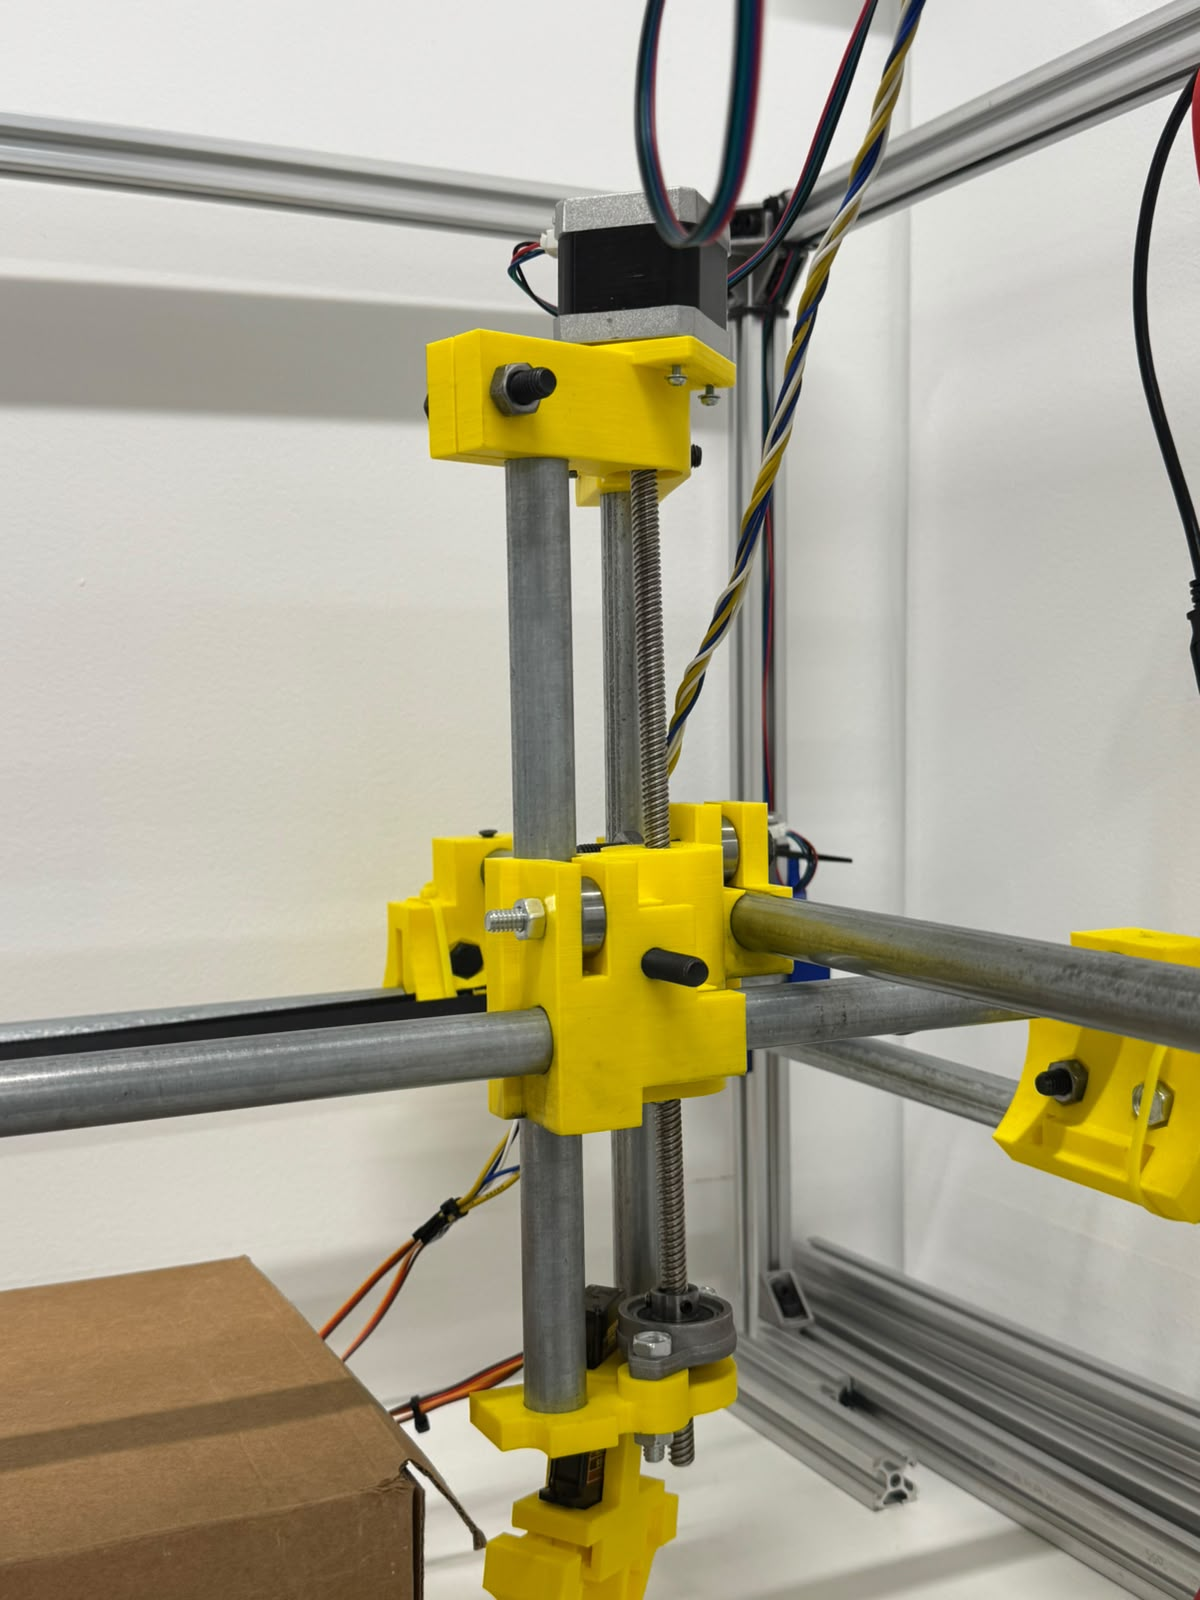
\includegraphics[width=0.55\textwidth,height=5.5cm,keepaspectratio]{Imagenes de Documentacion/F1_4.jpeg}
    \caption{Configuración inicial del mecanismo del eje Z.}
    \label{fig:fase1_eje_z}
    \par\small Fuente: elaboración propia.
\end{figure}

\begin{table}[H]
    \centering
    \caption{Observaciones de la evaluación mecánica inicial.}
    \label{tab:fase1_deficiencias}
    \begin{tabular}{p{0.08\textwidth}p{0.37\textwidth}p{0.43\textwidth}}
        \hline
        Eje & Configuración observada & Hallazgos de la inspección \\
        \hline
        X y Y & Carros impresos con rodamientos radiales sobre tubos metálicos. & Contacto plástico--tubo, resistencia al desplazamiento, desalineación y avance desigual de los extremos del pórtico. \\
        Z & Conjunto vertical con elementos de guiado y soportes impresos. & Desalineación del conjunto móvil y movimiento vertical irregular. \\
        \hline
    \end{tabular}
    \par\small\raggedright Fuente: elaboración propia a partir de la inspección visual y manual.
\end{table}

\section{Fase 2. Selección de componentes y rediseño mecánico}
\label{sec:resultados_fase2}

Se obtuvo un modelo CAD que conservó la arquitectura cartesiana y la disposición general de los ejes X, Y y Z. Se adaptaron los diseños de los soportes de las guías y de los motores de X y Y para incorporar ejes de acero de 12~mm de diámetro. La fabricación de las piezas correspondió a la fase siguiente.

El diseño incluyó cuatro carros para X y Y con rodamientos lineales con carcasa. Cada carro incorporó un paso perpendicular para el eje correspondiente, un espacio para el recorrido de la faja dentada y dos puntos adicionales de fijación (Figura~\ref{fig:fase2_carro_xy}).

\begin{figure}[H]
    \centering
    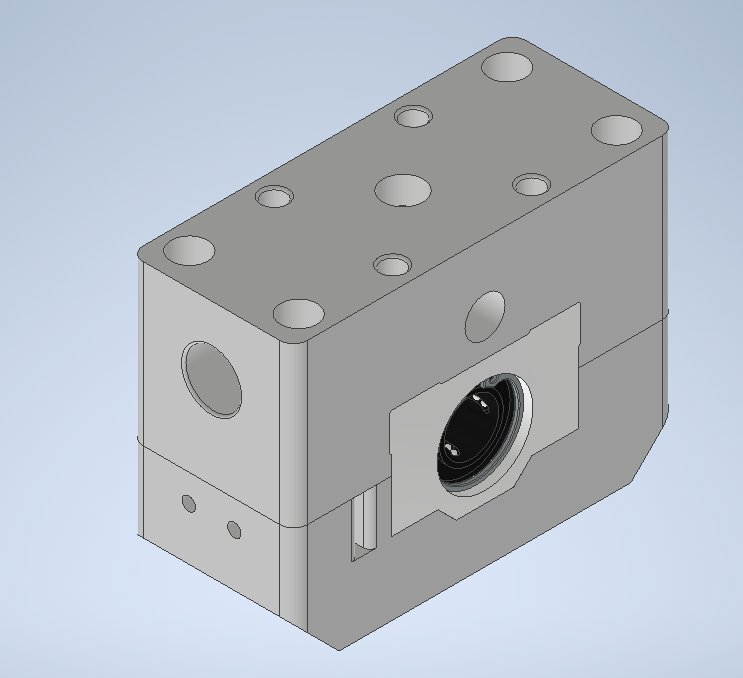
\includegraphics[width=0.65\textwidth,height=5.5cm,keepaspectratio]{Imagenes de Documentacion/F2_1.png}
    \caption{Modelo CAD del carro de traslación de los ejes X y Y.}
    \label{fig:fase2_carro_xy}
    \par\small Fuente: elaboración propia.
\end{figure}

El conjunto central incorporó rodamientos lineales cilíndricos para el desplazamiento en el plano XY. La intersección de ambos ejes quedó ubicada en el centro del conjunto y constituyó la referencia de montaje del mecanismo vertical (Figura~\ref{fig:fase2_centro_xy}).

\begin{figure}[H]
    \centering
    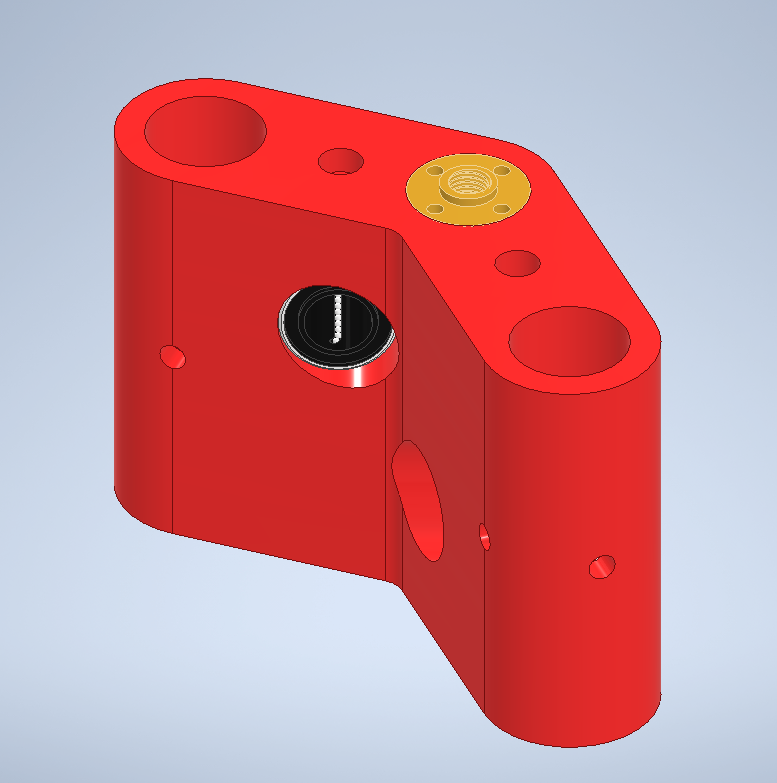
\includegraphics[width=0.65\textwidth,height=5.5cm,keepaspectratio]{Imagenes de Documentacion/F2_2.png}
    \caption{Modelo CAD del conjunto central del mecanismo cartesiano.}
    \label{fig:fase2_centro_xy}
    \par\small Fuente: elaboración propia.
\end{figure}

En el ensamblaje digital, Z incorporó dos guías y un tornillo de avance. Los soportes superior e inferior mantuvieron la separación entre centros definida en el conjunto central (Figura~\ref{fig:fase2_eje_z}). La integración de los componentes se documentó en el ensamblaje general de Autodesk Inventor (Figura~\ref{fig:fase2_ensamble_final}).

\begin{figure}[H]
    \centering
    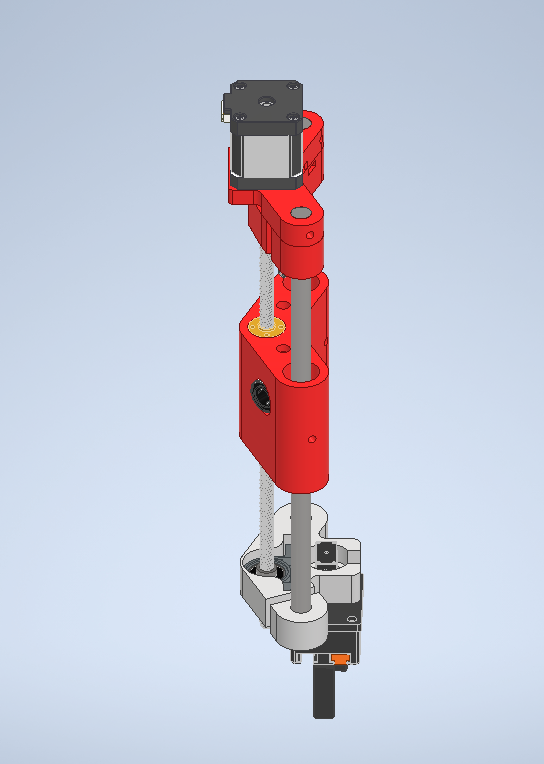
\includegraphics[width=0.60\textwidth,height=6cm,keepaspectratio]{Imagenes de Documentacion/F2_3.png}
    \caption{Modelo CAD del mecanismo vertical integrado al conjunto central.}
    \label{fig:fase2_eje_z}
    \par\small Fuente: elaboración propia.
\end{figure}

\begin{figure}[H]
    \centering
    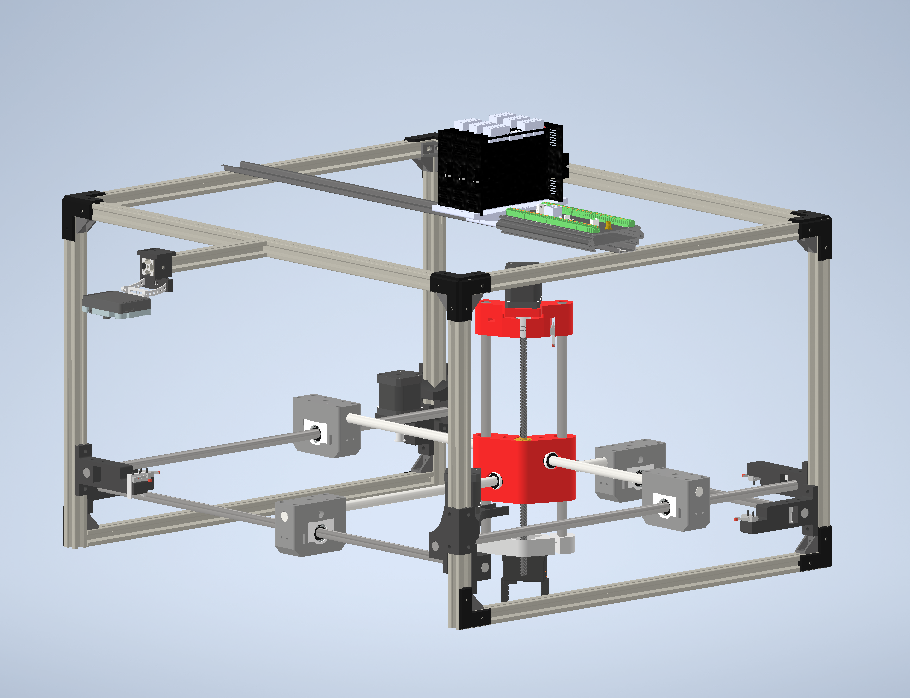
\includegraphics[width=0.75\textwidth,height=6cm,keepaspectratio]{Imagenes de Documentacion/F2_4.png}
    \caption{Ensamblaje CAD del brazo robótico cartesiano en Autodesk Inventor.}
    \label{fig:fase2_ensamble_final}
    \par\small Fuente: elaboración propia.
\end{figure}

% PENDIENTE: confirmar si las imágenes CAD correspondieron a la versión previa
% a fabricar o a una actualización posterior. No se les asignó una iteración.

\section{Fase 3. Implementación mecánica}
\label{sec:resultados_fase3}

\subsection{Componentes fabricados y configuración ensamblada}

Se incorporaron 48 piezas impresas en PLA, incluidas las escuadras de acabado estético. El consumo aproximado de material fue de 1.5~kg, incluidas las pruebas y las iteraciones de fabricación. Todas las piezas impresas se fabricaron nuevamente, incluso aquellas cuyos diseños se retomaron del mecanismo original.

Las piezas obtenidas incluyeron soportes de ejes guía, soportes de montaje de motores, carros de desplazamiento, piezas del conjunto central y soportes de Z. Parte de estos componentes se documentó en la Figura~\ref{fig:fase3_fabricacion}.

\begin{figure}[H]
    \centering
    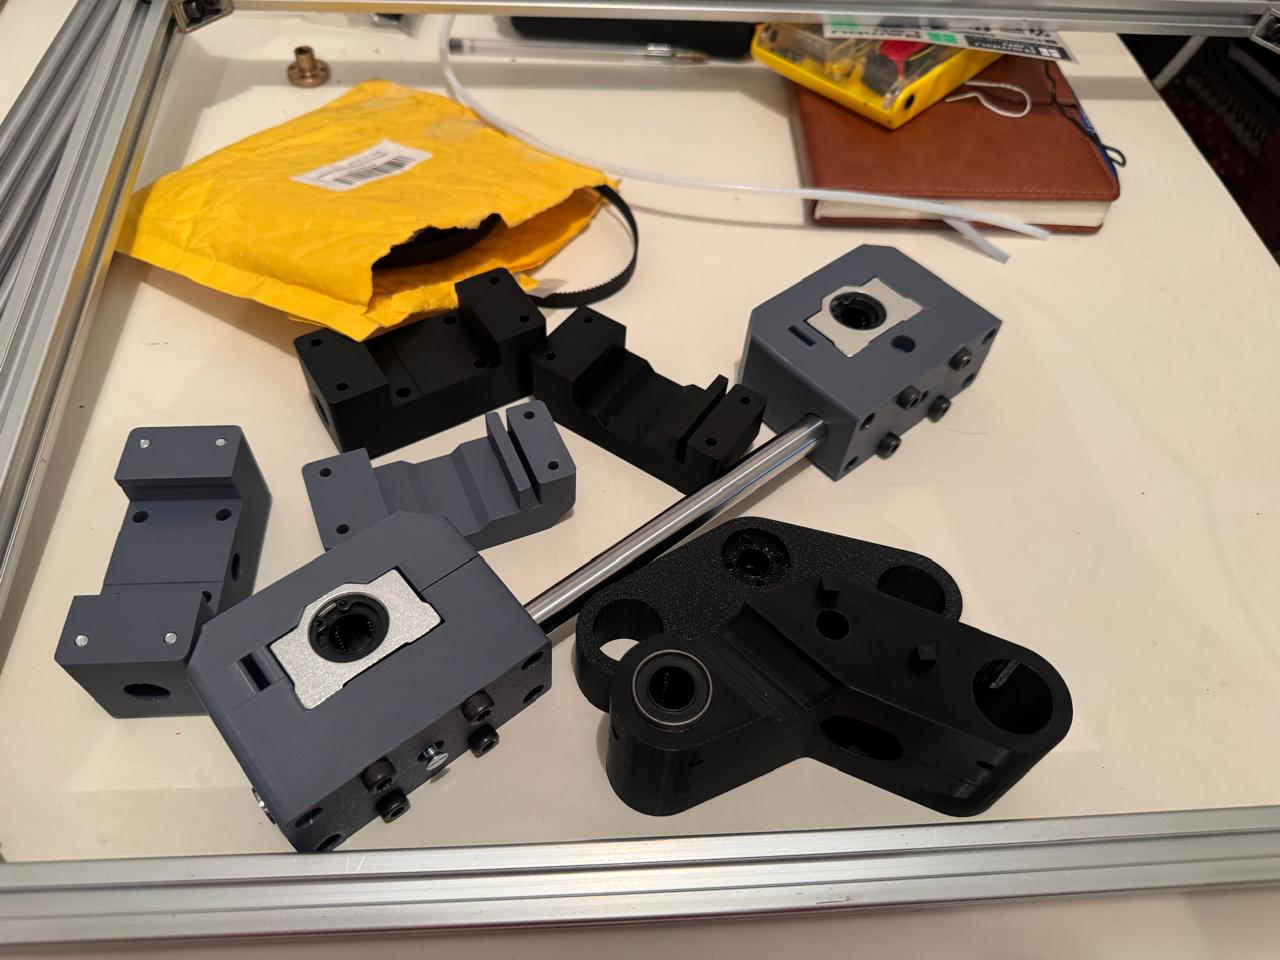
\includegraphics[width=0.72\textwidth,height=6cm,keepaspectratio]{figuras/fase3_componentes.jpeg}
    \caption{Componentes impresos y rodamientos preparados para el ensamblaje.}
    \label{fig:fase3_fabricacion}
    \par\small Fuente: elaboración propia.
\end{figure}

El conjunto ensamblado incorporó perfiles de aluminio 2020 de ranura en T, guías de acero de 12~mm, rodamientos lineales, fajas dentadas para X y Y y un tornillo de avance para Z. Las dimensiones y cantidades reportadas se organizaron en el Cuadro~\ref{tab:fase3_caracteristicas}.

\begin{table}[H]
    \centering
    \caption{Características del conjunto mecánico implementado.}
    \label{tab:fase3_caracteristicas}
    \begin{tabular}{p{0.53\textwidth}p{0.36\textwidth}}
        \hline
        Característica & Valor o configuración \\
        \hline
        Dimensiones generales de la estructura & $700 \times 580 \times 420$~mm \\
        Recorrido reportado del eje X\textsuperscript{a} & 446~mm \\
        Recorrido reportado del eje Y\textsuperscript{a} & 337~mm \\
        Recorrido del eje Z & \textit{Pendiente de medición} \\
        Diámetro de los ejes guía & 12~mm \\
        Ejes de 700~mm & 3 unidades \\
        Ejes de 580~mm & 3 unidades \\
        Perfiles estructurales & Aluminio 2020 de ranura en T \\
        Piezas impresas incorporadas & 48 unidades \\
        Material de las piezas impresas & PLA \\
        Consumo aproximado de PLA, incluidas las pruebas & 1.5~kg \\
        Transmisión en X y Y & Fajas dentadas \\
        Transmisión en Z & Tornillo de avance \\
        \hline
    \end{tabular}
    \par\small\raggedright Fuente: elaboración propia a partir de los datos de fabricación y ensamblaje del proyecto.
    \par\small La altura se refirió a la superficie de la mesa. El consumo de PLA incluyó las pruebas y no correspondió a la masa del brazo ensamblado.
    \par\small\textsuperscript{a} Se conservaron los valores reportados; su procedencia, del modelo CAD o de medición física, quedó pendiente de confirmación.
\end{table}

\subsection{Configuraciones del conjunto central y del soporte de la garra}

El conjunto central pasó por tres iteraciones. En las dos primeras se presentaron dificultades de retención de los rodamientos; en la configuración final estos permanecieron en sus alojamientos durante las comprobaciones de movimiento. Las configuraciones y sus observaciones se resumieron en el Cuadro~\ref{tab:fase3_iteraciones}.

\begin{table}[H]
    \centering
    \caption{Iteraciones del conjunto central y observaciones de montaje.}
    \label{tab:fase3_iteraciones}
    \begin{tabular}{p{0.10\textwidth}p{0.38\textwidth}p{0.40\textwidth}}
        \hline
        Iteración & Configuración & Observación \\
        \hline
        Primera & Cuerpo inicial al que se añadieron tornillos de presión. & Se observó la salida de los rodamientos de sus alojamientos antes de incorporar los tornillos. \\
        Segunda & Conjunto dividido en tres piezas con tornillos de presión. & Persistieron las dificultades de sujeción de los rodamientos. \\
        Tercera & Conjunto con tornillos de unión entre las piezas. & Los rodamientos permanecieron en sus alojamientos durante las comprobaciones realizadas. \\
        \hline
    \end{tabular}
    \par\small\raggedright Fuente: elaboración propia a partir de la descripción del proceso de fabricación y ensamblaje.
\end{table}

El conjunto central ensamblado y una vista del montaje parcial se documentaron en la Figura~\ref{fig:fase3_montaje}. El soporte inferior de Z incorporó una unión desmontable para la garra, en sustitución de la unión fija inicial. El efector final quedó ubicado en la intersección de los ejes del conjunto central.

\begin{figure}[H]
    \centering
    \begin{minipage}[b]{0.38\textwidth}
        \centering
        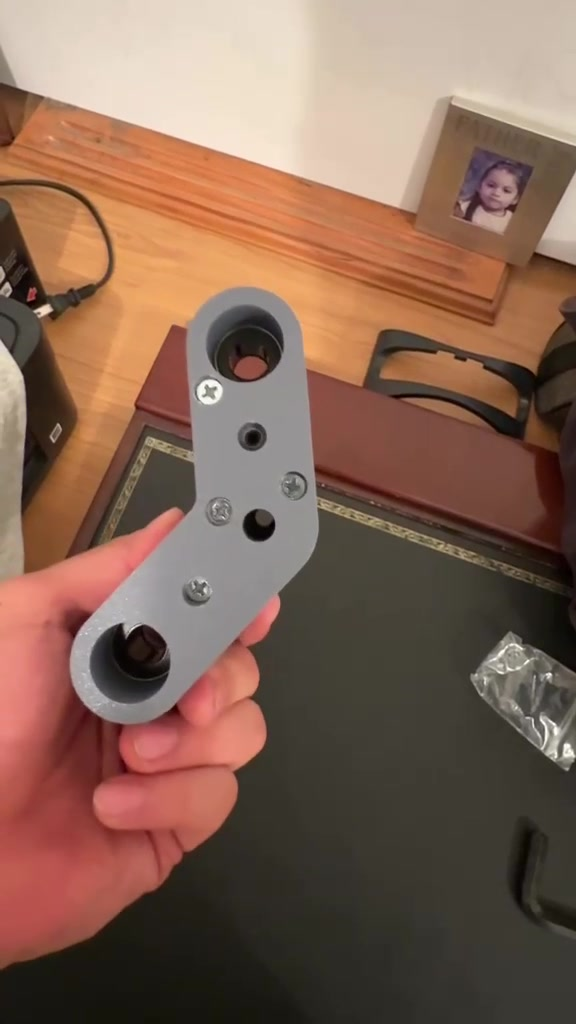
\includegraphics[width=\linewidth,height=6.5cm,keepaspectratio]{figuras/fase3_central_inferior.jpg}
        \par\small (a) Conjunto central ensamblado.
    \end{minipage}
    \hfill
    \begin{minipage}[b]{0.58\textwidth}
        \centering
        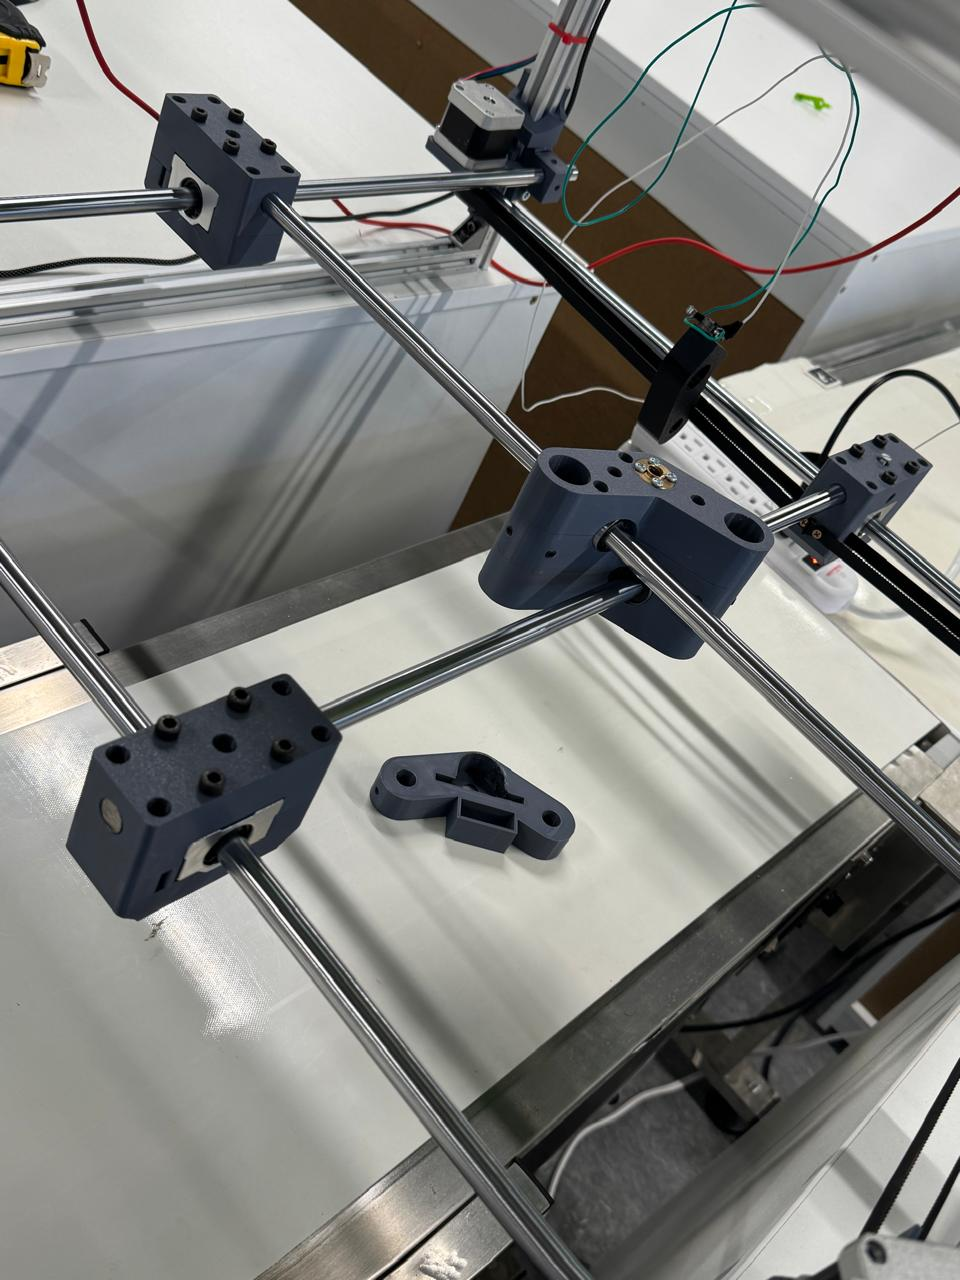
\includegraphics[width=\linewidth,height=6.5cm,keepaspectratio]{figuras/fase3_ensamblaje_parcial.jpeg}
        \par\small (b) Montaje parcial de guías y carros.
    \end{minipage}
    \caption{Conjunto central y montaje parcial del mecanismo cartesiano.}
    \label{fig:fase3_montaje}
    \par\small Fuente: elaboración propia; fotografía y fotograma del registro audiovisual del proyecto.
\end{figure}

\subsection{Comprobación mecánica preliminar}

Se comprobó el desplazamiento de los tres ejes mediante manipulación directa, antes del accionamiento electrónico. Los carros permanecieron sobre sus guías y no se reprodujeron los atascos identificados en el mecanismo original durante las comprobaciones realizadas.

La resistencia al movimiento se percibió menor que en el sistema original. El avance desigual de los extremos del pórtico resultó poco perceptible durante la inspección visual. Se observaron vibraciones leves y no se identificó deflexión de las guías a simple vista. Estas observaciones fueron cualitativas y no correspondieron a mediciones de precisión o repetibilidad.
